\documentclass[10pt,a4paper]{article}
\usepackage[margin=1.7cm]{geometry}
\usepackage{amsmath,amssymb}
\usepackage{tikz}
\usetikzlibrary{arrows.meta,positioning,shapes.geometric,fit,calc}
\usepackage[most]{tcolorbox}
\usepackage{booktabs,tabularx}
\usepackage{enumitem}
\usepackage{titlesec}
\usepackage{colortbl}
\usepackage[hidelinks]{hyperref}
\setlist{nosep,leftmargin=1.2em}
\setlength{\parindent}{0pt}
\setlength{\parskip}{3pt}
\titlespacing*{\section}{0pt}{8pt}{4pt}
\titlespacing*{\subsection}{0pt}{6pt}{2pt}

\definecolor{acc}{HTML}{2E5E8C}
\definecolor{warn}{HTML}{B5462E}
\definecolor{ok}{HTML}{2E7D4F}
\titleformat{\section}{\large\bfseries\color{acc}}{\thesection}{0.6em}{}
\titleformat{\subsection}{\normalsize\bfseries}{\thesubsection}{0.5em}{}

\newtcolorbox{keybox}[1][]{colback=acc!6,colframe=acc,boxrule=0.6pt,arc=2pt,left=4pt,right=4pt,top=2pt,bottom=2pt,fonttitle=\bfseries\small,#1}
\newtcolorbox{examtip}{colback=warn!6,colframe=warn,boxrule=0.6pt,arc=2pt,left=4pt,right=4pt,top=2pt,bottom=2pt,title=Exam tips,fonttitle=\bfseries\small}
\newtcolorbox{fixbox}{colback=gray!6,colframe=gray!60,boxrule=0.6pt,arc=2pt,left=4pt,right=4pt,top=2pt,bottom=2pt,title=Corrections to the notes / slides,fonttitle=\bfseries\small,coltitle=black}

\tikzset{
  box/.style={draw,rounded corners=2pt,align=center,font=\small,minimum height=7mm,inner sep=3pt},
  arr/.style={-{Stealth[length=2mm]},thick},
}
\newcommand{\hl}[1]{\cellcolor{warn!18}\textbf{#1}}
\newcommand{\ttx}[1]{\texttt{#1}}

\begin{document}

\begin{center}
{\LARGE\bfseries Cryptography \& Network Security}\\[2pt]
{\large Classical Encryption: Substitution, Transposition, Caesar \& Shift Ciphers}
\end{center}

\section{Classical Encryption Techniques}

Plaintext sent in the open over a channel invites attacks:
\textbf{passive} (eavesdropping, reading the data) and \textbf{active} (altering or injecting data).
Encryption turns plaintext into ciphertext so an interceptor learns nothing.

Classical techniques are \textbf{obsolete}: easy to break, keys recovered quickly. We study them because modern ciphers are built on the same two ideas: \emph{substitution} and \emph{transposition}.

\subsection{Substitution technique}
\begin{keybox}
Letters are \textbf{replaced} by other letters or symbols. Positions stay the same.
\end{keybox}
\begin{minipage}[t]{0.48\textwidth}
Key (a mapping table):\quad a$\to$M,\; b$\to$X,\; g$\to$A,\; x$\to$Z\\[3pt]
\begin{tabular}{@{}lccc@{}}
Plaintext  & b & a & g \\
           & $\downarrow$ & $\downarrow$ & $\downarrow$ \\
Ciphertext & \textbf{X} & \textbf{M} & \textbf{A}
\end{tabular}
\end{minipage}\hfill
\begin{minipage}[t]{0.48\textwidth}
\begin{itemize}
  \item The mapping table \emph{is} the key.
  \item Sender and receiver share the same table $\Rightarrow$ symmetric encryption.
\end{itemize}
\end{minipage}

\subsection{Transposition technique}
\begin{keybox}
Apply a \textbf{permutation}: the same letters are \textbf{rearranged}. No new letters appear.
\end{keybox}
Plaintext \ttx{NESO} $\to$ \ttx{ESON}, \ttx{SONE}, \ttx{ONES}, \ttx{ENOS}, \dots
\quad e.g.\ \ttx{ESON} takes letters in order $(2,3,4,1)$; \ttx{SONE} takes $(3,4,1,2)$.

A 4-letter word has only $4! = 24$ arrangements, so short messages are easy to guess.
Transposition is only effective for \textbf{long} plaintexts ($n!$ grows fast).

\subsection{Substitution vs.\ transposition}
\begin{center}\small
\begin{tabularx}{\textwidth}{@{}l X X@{}}
\toprule
 & \textbf{Substitution} & \textbf{Transposition} \\
\midrule
What changes & The letters themselves & The order of the letters \\
Positions & Unchanged & Permuted \\
Letters in ciphertext & New letters / symbols & Exactly the plaintext letters \\
Letter frequencies & Moved onto different symbols & Identical to plaintext \\
\bottomrule
\end{tabularx}
\end{center}

\begin{center}
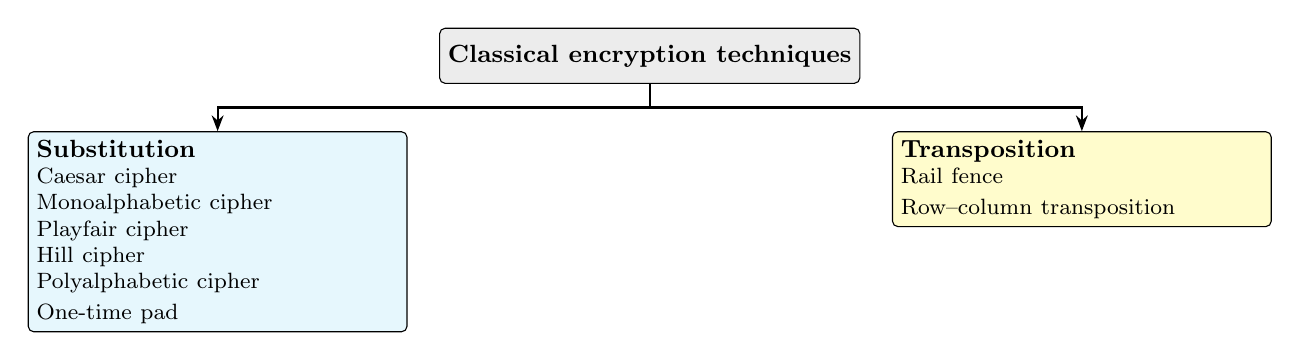
\begin{tikzpicture}[node distance=5mm]
  \node[box,fill=gray!15] (root) {\textbf{Classical encryption techniques}};
  \node[box,fill=cyan!10,below left=6mm and 4mm of root,text width=46mm,align=left] (sub) {\textbf{Substitution}\\
  \footnotesize Caesar cipher\\ \footnotesize Monoalphabetic cipher\\ \footnotesize Playfair cipher\\ \footnotesize Hill cipher\\ \footnotesize Polyalphabetic cipher\\ \footnotesize One-time pad};
  \node[box,fill=yellow!20,below right=6mm and 4mm of root,text width=46mm,align=left] (tra) {\textbf{Transposition}\\
  \footnotesize Rail fence\\ \footnotesize Row--column transposition};
  \draw[arr] (root.south) -- ++(0,-3mm) -| (sub.north);
  \draw[arr] (root.south) -- ++(0,-3mm) -| (tra.north);
\end{tikzpicture}
\end{center}

\section{Caesar Cipher}

\begin{keybox}
Earliest and simplest substitution cipher, used by Julius Caesar. Replace each letter with the letter \textbf{three places further down} the alphabet, wrapping from \ttx{z} back to \ttx{a}.
\end{keybox}

\subsection{Letters as numbers (start at 0)}
\begin{center}\small\setlength{\tabcolsep}{4pt}
\begin{tabular}{*{13}{c}}
\toprule
A&B&C&D&E&F&G&H&I&J&K&L&M\\
0&1&2&3&4&5&6&7&8&9&10&11&12\\
\midrule
N&O&P&Q&R&S&T&U&V&W&X&Y&Z\\
13&14&15&16&17&18&19&20&21&22&23&24&25\\
\bottomrule
\end{tabular}
\end{center}
Numbering from 0 matches the remainders mod 26, which are exactly $0,1,\dots,25$.

\subsection{Algorithm}
\begin{minipage}[c]{0.55\textwidth}
\begin{keybox}[title=Encryption and decryption]
\vspace{-6pt}
\begin{align*}
C &= E(p,k) = (p + k) \bmod 26\\
p &= D(C,k) = (C - k) \bmod 26
\end{align*}
Caesar cipher: $k = 3$.
\end{keybox}
\begin{itemize}
  \item $p$ = plaintext letter's number, $C$ = ciphertext letter's number, $k$ = key (shift).
  \item Convention: plaintext in lowercase, ciphertext in UPPERCASE.
  \item \textbf{mod gives the remainder, not the quotient.} $27 \bmod 26 = 1$.
  \item Negative during decryption? Add 26. \;$-2 \bmod 26 = 24$.
\end{itemize}
\end{minipage}\hfill
\begin{minipage}[c]{0.42\textwidth}
\centering
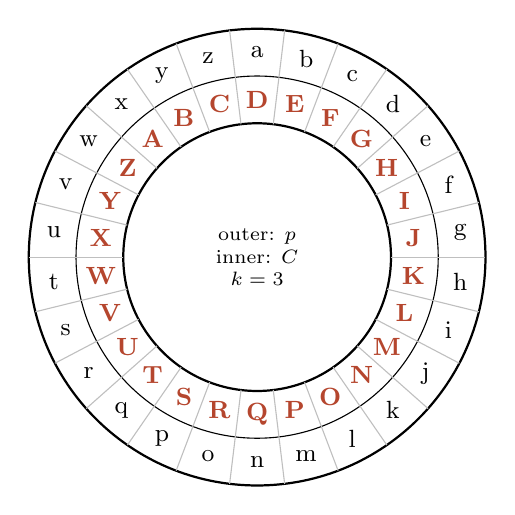
\begin{tikzpicture}
  \draw[thick] (0,0) circle (2.9);
  \draw (0,0) circle (2.3);
  \draw[thick] (0,0) circle (1.7);
  \foreach \pl/\cl [count=\n from 0] in {a/D,b/E,c/F,d/G,e/H,f/I,g/J,h/K,i/L,j/M,k/N,l/O,m/P,n/Q,o/R,p/S,q/T,r/U,s/V,t/W,u/X,v/Y,w/Z,x/A,y/B,z/C}{
    \pgfmathsetmacro{\ang}{90-\n*360/26}
    \pgfmathsetmacro{\sep}{\ang+180/26}
    \node[font=\small] at (\ang:2.6) {\pl};
    \node[font=\small\bfseries,text=warn] at (\ang:2.0) {\cl};
    \draw[gray!50] (\sep:1.7) -- (\sep:2.9);
  }
  \node[font=\scriptsize,align=center] at (0,0) {outer: $p$\\inner: $C$\\$k=3$};
\end{tikzpicture}
\end{minipage}

\subsection{Worked example: encrypt ``neso academy'' ($k=3$)}
\begin{center}\small\setlength{\tabcolsep}{5pt}
\begin{tabular}{@{}l*{4}{c}|*{7}{c}@{}}
\toprule
Plaintext & n&e&s&o & a&c&a&d&e&m&y\\
$p$ & 13&4&18&14 & 0&2&0&3&4&12&24\\
$p+3$ & 16&7&21&17 & 3&5&3&6&7&15&\hl{27}\\
$\bmod 26$ & 16&7&21&17 & 3&5&3&6&7&15&\hl{1}\\
Ciphertext & \textbf{Q}&\textbf{H}&\textbf{V}&\textbf{R} & \textbf{D}&\textbf{F}&\textbf{D}&\textbf{G}&\textbf{H}&\textbf{P}&\textbf{B}\\
\bottomrule
\end{tabular}
\end{center}
Answer: \textbf{\ttx{QHVR DFDGHPB}}.
The only wrap-around is \ttx{y}: $24+3 = 27$, and $27 = 26\times 1 + \mathbf{1}$, so $C = 1 = $ \ttx{B}.
(Counting on: y $\to$ z $\to$ a $\to$ \textbf{b}.) For the other letters you can just count three letters forward.

\subsection{Homework 1: decrypt ``QHWZRUN VHFXULWB'' ($k=3$)}
\begin{center}\small\setlength{\tabcolsep}{3.6pt}
\begin{tabular}{@{}l*{7}{c}|*{8}{c}@{}}
\toprule
Ciphertext & Q&H&W&Z&R&U&N & V&H&F&X&U&L&W&B\\
$C$ & 16&7&22&25&17&20&13 & 21&7&5&23&20&11&22&1\\
$C-3$ & 13&4&19&22&14&17&10 & 18&4&2&20&17&8&19&\hl{$-2$}\\
$\bmod 26$ & 13&4&19&22&14&17&10 & 18&4&2&20&17&8&19&\hl{24}\\
Plaintext & n&e&t&w&o&r&k & s&e&c&u&r&i&t&y\\
\bottomrule
\end{tabular}
\end{center}
Answer: \textbf{network security}. Note the last letter: $1-3=-2$, add 26 $\Rightarrow 24 =$ \ttx{y}.

\section{Shift Cipher (the general form)}

\begin{keybox}
Same formulas, but the key $k$ can be any of $1,2,\dots,25$. \textbf{Caesar cipher = shift cipher with $k=3$.}
\end{keybox}
\begin{itemize}
  \item $k=0$ is useless: $C = (p+0) \bmod 26 = p$, so the ciphertext equals the plaintext. (Homework: ``Neso'', $k=0$ $\Rightarrow$ \ttx{NESO}.)
  \item $k=26$ is the same as $k=0$. So there are only \textbf{25 usable keys}.
\end{itemize}

\textbf{Example:} ``Neso'', $k=4$: \;
N $13{+}4{=}17\to$\textbf{R},\;
e $4{+}4{=}8\to$\textbf{I},\;
s $18{+}4{=}22\to$\textbf{W},\;
o $14{+}4{=}18\to$\textbf{S} \;$\Rightarrow$\; \textbf{\ttx{RIWS}}.

\textbf{Homework 2:} ``cryptography'', $k=4$:
\begin{center}\small\setlength{\tabcolsep}{4.5pt}
\begin{tabular}{@{}l*{12}{c}@{}}
\toprule
Plaintext & c&r&y&p&t&o&g&r&a&p&h&y\\
$p$ & 2&17&24&15&19&14&6&17&0&15&7&24\\
$p+4 \bmod 26$ & 6&21&\hl{2}&19&23&18&10&21&4&19&11&\hl{2}\\
Ciphertext & G&V&C&T&X&S&K&V&E&T&L&C\\
\bottomrule
\end{tabular}
\end{center}
Answer: \textbf{\ttx{GVCTXSKVETLC}} (both \ttx{y}'s wrap: $24+4=28 \equiv 2$).

\textbf{In code:} the 0--25 numbering is a convention. With ASCII (\ttx{A}=65, \ttx{a}=97), shift to 0 first, then back:
\;$C = \big((p - 65 + k) \bmod 26\big) + 65$ for uppercase (use 97 for lowercase).

\subsection{Pros and cons of the Caesar cipher}
\begin{minipage}[t]{0.3\textwidth}
\textbf{Pros}
\begin{enumerate}[leftmargin=1.5em]
  \item Simple.
  \item Easy to implement.
\end{enumerate}
\end{minipage}\hfill
\begin{minipage}[t]{0.66\textwidth}
\textbf{Cons}
\begin{enumerate}[leftmargin=1.5em]
  \item The encryption and decryption algorithms are known.
  \item Only 25 keys to try $\Rightarrow$ vulnerable to \textbf{brute-force attack}.
  \item The plaintext language is known and easily recognisable, so you can tell when you have hit the right key.
\end{enumerate}
\end{minipage}

\section{Brute-Force Attack on the Caesar/Shift Cipher}

\begin{keybox}
\textbf{Brute force}: try every possible key until readable plaintext appears. With 25 keys this takes seconds by hand.
\end{keybox}

Ciphertext: \ttx{SQDYMZK}. Shift every letter forward by 0, 1, 2, \dots, 25 and look for a real word:

\begin{center}\small\ttfamily\setlength{\tabcolsep}{6pt}
\begin{tabular}{@{}ccl@{}}
\toprule
\rmfamily\bfseries Fwd & \rmfamily\bfseries Back & \rmfamily\bfseries Result\\
\midrule
0 & 26 & SQDYMZK\\
1 & 25 & TREZNAL\\
2 & 24 & USFAOBM\\
3 & 23 & VTGBPCN\\
4 & 22 & WUHCQDO\\
5 & 21 & XVIDREP\\
6 & 20 & YWJESFQ\\
7 & 19 & ZXKFTGR\\
8 & 18 & AYLGUHS\\
9 & 17 & BZMHVIT\\
10 & 16 & CANIWJU\\
11 & 15 & DBOJXKV$^\ast$\\
12 & 14 & ECPKYLW\\
\bottomrule
\end{tabular}
\qquad
\begin{tabular}{@{}ccl@{}}
\toprule
\rmfamily\bfseries Fwd & \rmfamily\bfseries Back & \rmfamily\bfseries Result\\
\midrule
13 & 13 & FDQLZMX\\
\rowcolor{warn!18} \textbf{14} & \textbf{12} & \textbf{GERMANY}\\
15 & 11 & HFSNBOZ\\
16 & 10 & IGTOCPA\\
17 & 9 & JHUPDQB\\
18 & 8 & KIVQERC\\
19 & 7 & LJWRFSD\\
20 & 6 & MKXSGTE\\
21 & 5 & NLYTHUF\\
22 & 4 & OMZUIVG$^\ast$\\
23 & 3 & PNAVJWH\\
24 & 2 & QOBWKXI\\
25 & 1 & RPCXLYJ\\
\bottomrule
\end{tabular}
\end{center}
{\footnotesize $^\ast$ Recomputed; the notes had these rows slightly wrong (see corrections box).}

\begin{itemize}
  \item Forward $+$ back $= 26$, because shifting forward 14 is the same as shifting back 12: $\;C + 14 \equiv C - 12 \pmod{26}$.
  \item Only one row is English: \textbf{GERMANY}. The attacker now has the plaintext \emph{and} the key.
  \item \textbf{Which number is the key?} The sender encrypted with $k = \mathbf{12}$ (G $6+12=18=$ S, \dots, Y $24+12=36\equiv10=$ K). The 14 is the forward shift that \emph{undoes} it. The lecture calls 14 ``the key''; be clear which one you mean in an exam.
\end{itemize}

\begin{keybox}[title=Decryption vs.\ cryptanalysis]
\textbf{Decryption}: the receiver \emph{has} the key and reverses the encryption.\\
\textbf{Cryptanalysis}: an attacker \emph{without} the key recovers the plaintext and/or the key (e.g.\ by brute force).
\end{keybox}

\begin{examtip}
\begin{itemize}
  \item Substitution = replace letters; transposition = rearrange letters. Know the list of ciphers under each.
  \item Write both formulas: $C=(p+k)\bmod 26$, $p=(C-k)\bmod 26$. Caesar is $k=3$.
  \item Always show the wrap-around step (e.g.\ $27 \bmod 26 = 1$) and fix negatives by adding 26.
  \item Key space is 25 (not 26): $k=0$ changes nothing.
  \item Three cons of Caesar: algorithms known, only 25 keys, language recognisable.
  \item For brute force: draw the table, box the readable row, state the key.
\end{itemize}
\end{examtip}

\begin{fixbox}
\begin{itemize}
  \item ``neso academy'' encrypts to \ttx{QHVR DFDGHPB}. The notes' final answer \ttx{QHVRDFDGHB} drops the \ttx{P}.
  \item Brute-force table: row 11 is \ttx{DBOJXKV} and row 22 is \ttx{OMZUIVG}. Row 12 (\ttx{ECPKYLW}) was already correct.
  \item The notes call con \#1 a ``Kerckhoffs violation''. It isn't: public algorithms are normal (see the intro sheet). The problem is a public algorithm \emph{plus} only 25 keys.
  \item Slide typo: ``used \emph{be} Julius Caesar'' $\to$ ``used \emph{by}''.
\end{itemize}
\end{fixbox}

\end{document}
